\documentclass[main.tex]{subfiles}

\begin{document}

\subsection{Area di studio: inquadramento territoriale}

L’area di studio coinvolge 11 regioni italiane e per ognuna di esse il Progetto BeeNet ha identificato 2 siti (Fig. \ref{fig:Area}), dove per mezzo di appositi transetti sono state identificate le piante di interesse entomofilo.

\begin{figure}[H]
\centering
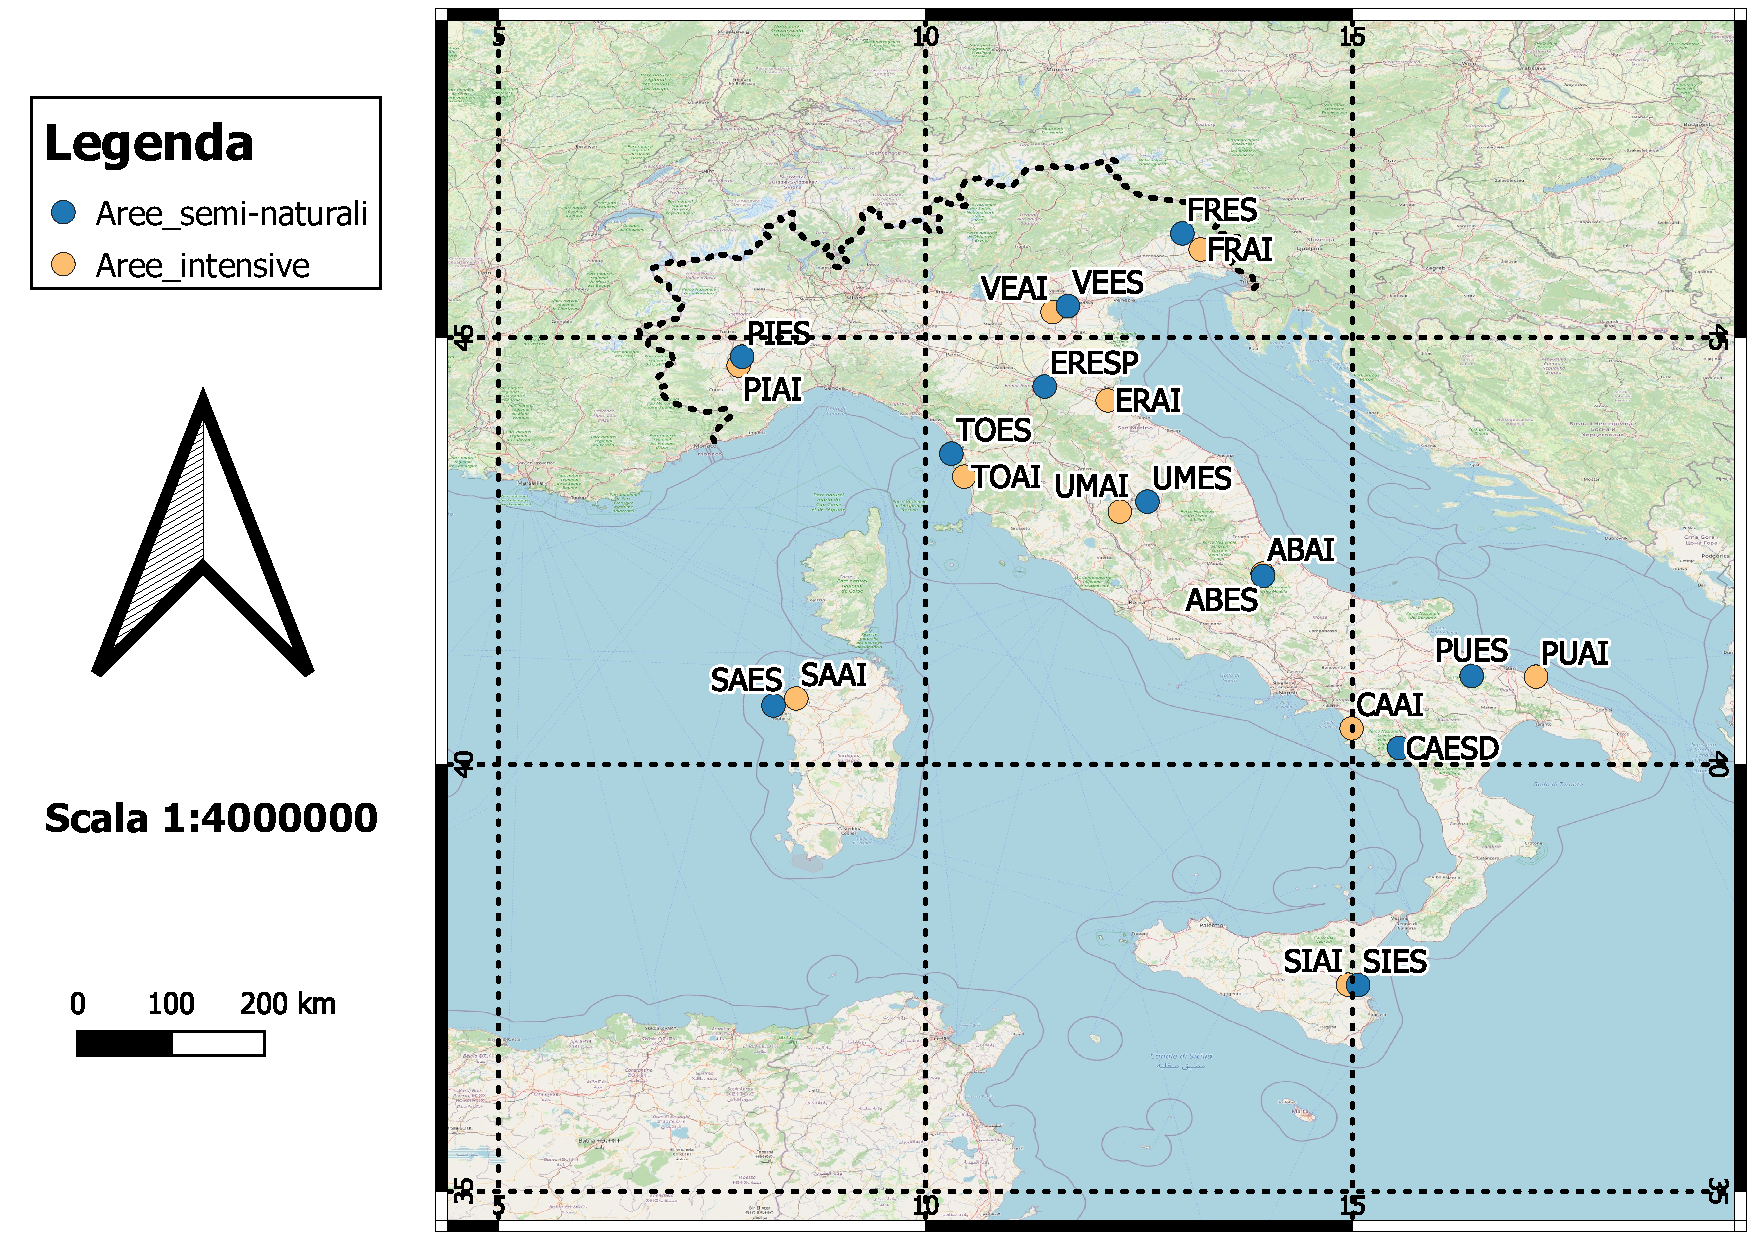
\includegraphics[width=0.9\textwidth]{./Immagini/Area_di_studio}
\caption{Mappa dei siti realizzata tramite QGIS.}
\label{fig:Area}
\end{figure}

I siti sono compresi in un’altitudine che varia da 0-500 m s.l.m. e in ogni regione sono definite 2 tipologie di agroecosistema (Fig. \ref{fig:Corine}). I suddetti siti, identificabili tramite apposito nominativo, consistono in un agro-ecosistema intensivo (suffisso -AI) e un agro-ecosistema seminaturale situato all’interno di un’area protetta (suffisso –ES) al fine di confrontare la biodiversità dei siti, la composizione dell'ambiente e di conseguenza la stabilità delle comunità composte da piante e impollinatori.
Si definisce agroecosistema intensivo una zona altamente antropizzata al fine di massimizzare la produzione del sistema agricolo, con il minore sforzo e costo, ed è basata sulla specializzazione in poche o addirittura singole colture. In queste zone vi è un ampio utilizzo di macchinari per la lavorazione del terreno, fertilizzanti e fitofarmaci che modificano pesantemente il servizio ecosistemico. In questa tipologia di agricoltura l’uniformità e l’omogeneità dei grandi campi di monocolture sono incompatibili con la qualità ambientale e la conservazione delle risorse biologiche.
Per agro-ecosistema seminaturale si intende un habitat parzialmente occupato da siti agricoli, dove si crea una condizione di frammentazione del paesaggio influenzando di conseguenza la biodiversità e la sostenibilità dell’ecosistema stesso. Di particolare significato, in questo processo di frammentazione, è la creazione di aree di contatto tra ecotopi differenti, per cui si creano brusche aree di passaggio, definite “ecotoni”, dove la eterogeneità della condizione fisica crea i presupposti per un accrescimento di biodiversità.
Le aree sono scelte secondo le categorie di uso del suolo CORINE \citep{corine}, emanato dal Consiglio delle Comunità Europee al fine di omogeneizzare le informazioni territoriali sullo stato dell'ambiente e fornire supporto per lo sviluppo di politiche comuni e controllarne gli effetti. In questo caso, CORINE Land Cover (CLC), è specifico per il rilevamento e il monitoraggio delle caratteristiche di copertura e uso del territorio, con particolare attenzione alle esigenze di tutela.
L’analisi dei dati italiani secondo il CLC2018 di quarto livello determina che i siti in agroecosistema intensivo sono stati scelti all’interno della categoria 2.1.1.1, tale classe oltre ad identificarsi nella categoria delle ‘colture intensive’ presenta la maggior copertura sul territorio nazionale (24\%). Mentre per i siti in zone seminaturali sono state rispettivamente scelte le categorie 2.4.2 e 2.4.3, che identificano la prima classe in ‘sistemi colturali e particellari complessi’ e la seconda in ‘aree prevalentemente occupate da colture agrarie con presenza di spazi naturali importanti’; entrambe presentano una copertura del 7\% sul territorio nazionale \citep{muna}.
Nel caso degli agro-ecosistemi seminaturali è riportato il nominativo dell’area protetta in cui è ubicato il sito e dunque dove è avvenuta l’identificazione delle piante entomofile.

\begin{figure}[H]
\centering
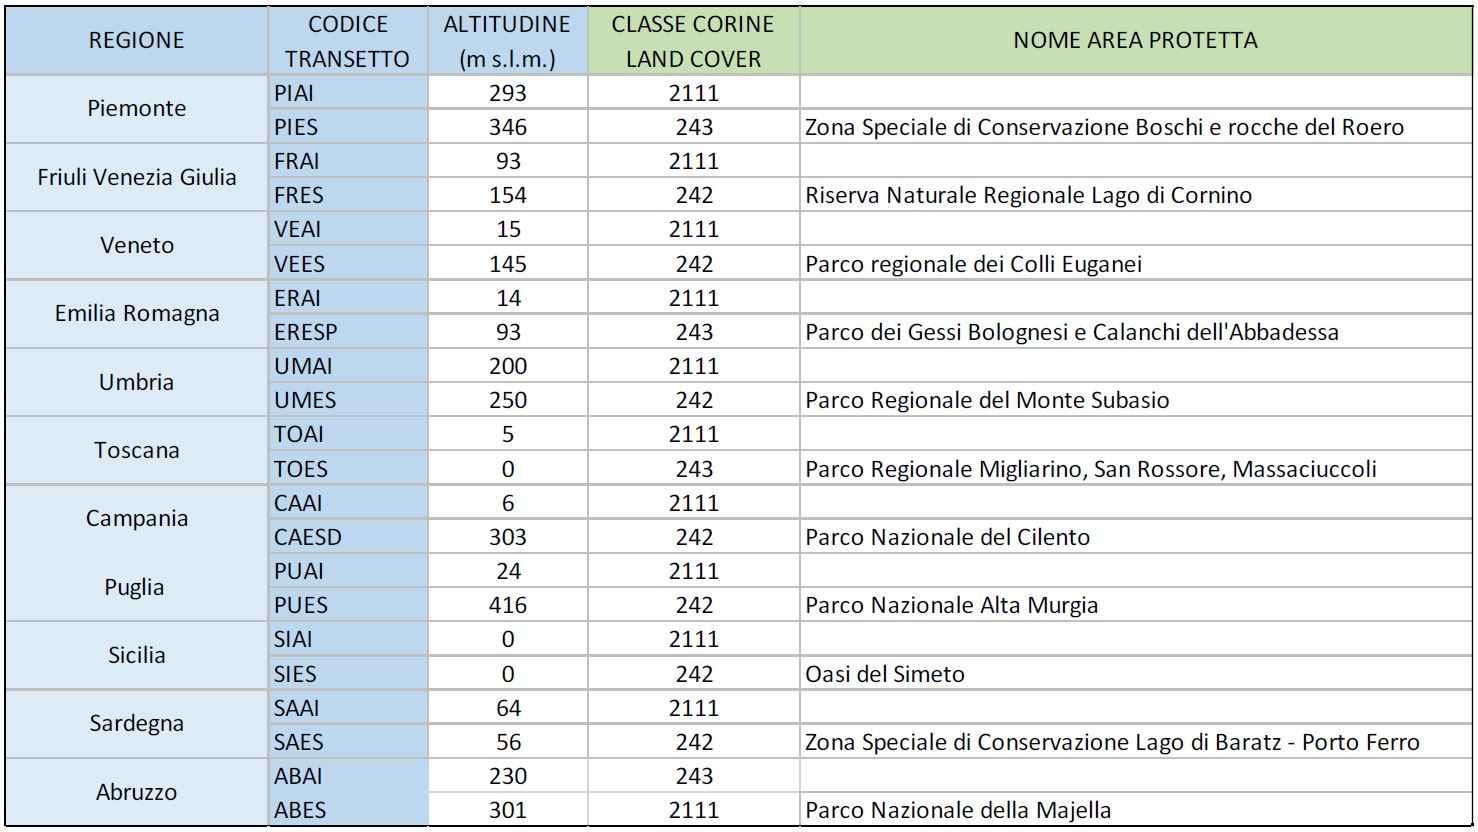
\includegraphics[width=0.9\textwidth]{./Immagini/Corine.JPG}
\caption{dati e valori relativi ai siti di studio BeeNet.}
\label{fig:Corine}
\end{figure}

\end{document}